\documentclass[ru, listings]{labreport}
\subject{Организация ЭВМ и систем}
\titleparts{Лабораторная работа №1}{Вариант 9}
\students{Нестеров Дали \\[1mm] Лабушев Тимофей}

\begin{document}

\maketitlepage

\section*{Цель работы}

Ознакомиться с интегрированной средой программирования keil-C и получить навыки работы
с текстовым редактором этой программы. Получить навыки работы с программными проектами
интегрированной среды программирования keil-C для микроконтроллеров семейства MCS-51.
Научиться транслировать программы, написанными на языке программирования C-51,
и получать загрузочные файлы микроконтроллера.
Ознакомиться с основами работы отладчика программ в
интегрированной среде программирования keil-C и получить навыки работы с ним.

\section*{Исходный текст программы}

\lstinputlisting[language=c, basicstyle=\scriptsize]{source.c}

\section*{Cтруктура программного проекта}

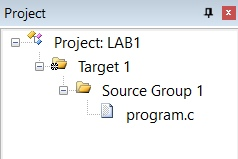
\includegraphics[width=0.25\textwidth]{project-structure}

\section*{Порядок создания загрузочного модуля}

\section*{Файл листинга}

\lstinputlisting[basicstyle=\scriptsize]{listing.asm}

\section*{Распечатка загрузочного файл}

\lstinputlisting[basicstyle=\scriptsize]{boot.hex}

\section*{Пошаговые значения переменных \texttt{I}, \texttt{A[I]}, \texttt{S}}

\begin{tabular}{|c|c|c|}
  \hline
  \verb|I| & \verb|A[I]| & \verb|S| \\\hline
  1 & 5 & 0 \\
  2 & -8 & -8 \\
  3 & 7 & -8 \\
  4 & -3 & -11 \\
  5 & 15 & -11 \\
  6 & 38 & -11 \\
  7 & -11 & -22 \\
  8 & 66 & -22 \\
  9 & -6 & -28 \\\hline
\end{tabular}

\section*{Выводы}

\end{document}
